% If I Invest Tomorrow — Final review presentation
% Build:  tectonic final_review.tex        (or: xelatex final_review.tex)
% Figures: python presentation/make_figures.py   (regenerates figures/ from the engine)
\documentclass[aspectratio=169,11pt]{beamer}

% ------------------------------------------------------------------ packages
\usepackage{fontspec}
\usepackage{graphicx}
\usepackage{booktabs}
\usepackage{colortbl}
\usepackage{tabularx}
\usepackage{array}
\usepackage{amsmath}
\usepackage{tikz}
\usetikzlibrary{positioning,arrows.meta,fit,calc}

% ------------------------------------------------------------------ fonts
\defaultfontfeatures{Ligatures=TeX}
\setsansfont{SourceSansPro}[Extension=.otf, UprightFont=*-Regular, BoldFont=*-Semibold,
  ItalicFont=*-RegularIt, BoldItalicFont=*-SemiboldIt]
\newfontfamily\displayfont{LibertinusSerif}[Extension=.otf, UprightFont=*-Regular, ItalicFont=*-Italic, BoldFont=*-Semibold]
\newfontfamily\numfont{SourceSansPro}[Extension=.otf, UprightFont=*-Regular, BoldFont=*-Semibold, Numbers={Lining,Monospaced}]
\usefonttheme{professionalfonts}
\geometry{papersize={20cm,11.25cm}}

% ------------------------------------------------------------------ colours (match the web app)
\definecolor{paper}{HTML}{F5F4EF}
\definecolor{surface}{HTML}{FBFAF7}
\definecolor{ink}{HTML}{17160F}
\definecolor{muted}{HTML}{6B685E}
\definecolor{faint}{HTML}{9B978B}
\definecolor{rulec}{HTML}{D6D2C6}
\definecolor{border}{HTML}{E0DDD3}
\definecolor{brand}{HTML}{0E5A43}
\definecolor{pos}{HTML}{157046}
\definecolor{neg}{HTML}{B3361F}
\definecolor{caution}{HTML}{9A6400}
\definecolor{cA}{HTML}{2A78D6}
\definecolor{cB}{HTML}{EB6834}
\definecolor{cC}{HTML}{1BAF7A}
\definecolor{cD}{HTML}{EDA100}
\definecolor{cE}{HTML}{E87BA4}
\definecolor{cG}{HTML}{4A3AA7}

% ------------------------------------------------------------------ theme
\setbeamercolor{background canvas}{bg=paper}
\setbeamercolor{normal text}{fg=ink}
\setbeamercolor{structure}{fg=ink}
\setbeamercolor{alerted text}{fg=brand}
\setbeamercolor{itemize item}{fg=faint}
\setbeamercolor{itemize subitem}{fg=faint}
\setbeamercolor{enumerate item}{fg=brand}
\setbeamertemplate{navigation symbols}{}
\setbeamertemplate{itemize item}{\raisebox{0.25ex}{\color{faint}\rule{0.42em}{0.42em}}}
\setbeamertemplate{itemize subitem}{\raisebox{0.3ex}{\color{faint}\rule{0.3em}{0.3em}}}
\setbeamertemplate{enumerate item}{\color{brand}\insertenumlabel.}
\setlength{\leftmargini}{1.1em}
\setbeamersize{text margin left=1.25cm, text margin right=1.25cm}
\setbeamerfont{normal text}{size=\normalsize}

% section eyebrow + serif title
\setbeamertemplate{frametitle}{%
  \vspace*{0.55cm}%
  {\usebeamerfont{frametitle}\fontsize{7.5}{9}\selectfont\color{brand}\addfontfeature{LetterSpace=12}\MakeUppercase{\insertsectionhead}\par}%
  \vspace*{0.12cm}%
  {\displayfont\fontsize{22}{25}\selectfont\color{ink}\insertframetitle\par}%
  \ifx\insertframesubtitle\@empty\else{\fontsize{10}{12}\selectfont\color{muted}\insertframesubtitle\par}\fi
  \vspace*{0.05cm}%
}
\makeatletter
\setbeamertemplate{footline}{%
  \hspace*{1.25cm}{\color{rulec}\rule{\dimexpr\paperwidth-2.5cm\relax}{0.4pt}}\par
  \vspace*{0.16cm}%
  \hspace*{1.25cm}%
  \parbox[t]{\dimexpr\paperwidth-2.5cm\relax}{\fontsize{7}{8}\selectfont\color{faint}%
    If I Invest Tomorrow \enspace·\enspace 23CSE322 Financial Engineering \enspace·\enspace Team 01\hfill\insertframenumber\,/\,\inserttotalframenumber}%
  \vspace*{0.32cm}%
}
\makeatother

% ------------------------------------------------------------------ helpers
\newcommand{\eyebrow}[1]{{\fontsize{7.5}{9}\selectfont\color{muted}\addfontfeature{LetterSpace=10}\MakeUppercase{#1}}}
\newcommand{\muted}[1]{\leavevmode{\color{muted}#1}}
\newcommand{\faint}[1]{\leavevmode{\color{faint}#1}}
\newcommand{\up}[1]{\leavevmode{\color{pos}#1}}
\newcommand{\dn}[1]{\leavevmode{\color{neg}#1}}
% screenshot with a hairline frame
\newcommand{\shot}[2]{\tikz\node[inner sep=0pt, draw=border, line width=0.6pt, rounded corners=2pt]{\includegraphics[#1]{#2}};}
\newcommand{\swatch}[1]{\textcolor{#1}{\rule{0.55em}{0.55em}}}
\newcommand{\hair}{{\color{rulec}\rule{\linewidth}{0.4pt}}}
% big figure: value + label
\newcommand{\kpi}[3][ink]{%
  \begin{minipage}[t]{\linewidth}
    {\fontsize{6.8}{8}\selectfont\color{muted}\addfontfeature{LetterSpace=10}\MakeUppercase{#3}\par}\vspace{2pt}
    {\numfont\fontsize{17}{19}\selectfont\color{#1}#2\par}
  \end{minipage}}
\newcolumntype{R}{>{\raggedleft\arraybackslash}X}
\newcolumntype{L}{>{\raggedright\arraybackslash}X}
\newcommand{\thd}[1]{\leavevmode{\fontsize{7}{8}\selectfont\color{muted}\addfontfeature{LetterSpace=8}\MakeUppercase{#1}}}
\renewcommand{\arraystretch}{1.18}
\setlength{\aboverulesep}{0pt}\setlength{\belowrulesep}{0pt}
\newcommand{\tabrule}{\arrayrulecolor{rulec}\midrule}
\newcommand{\toprl}{\arrayrulecolor{rulec}\toprule}
\newcommand{\botrl}{\arrayrulecolor{rulec}\bottomrule}

% callout with a green left rule
\newenvironment{callout}{%
  \begin{tikzpicture}\node[inner sep=0pt, text width=\linewidth-12pt](n)\bgroup\small}%
  {\egroup;\draw[brand, line width=1.6pt]($(n.north west)+(-7pt,0)$)--($(n.south west)+(-7pt,0)$);\end{tikzpicture}}

\tikzset{
  box/.style={draw=border, fill=surface, rounded corners=3pt, line width=0.5pt, align=center, font=\fontsize{8}{9.5}\selectfont, inner sep=5pt,
    execute at begin node={\hyphenpenalty=10000\exhyphenpenalty=10000}},
  sbox/.style={box, fill=paper},
  hl/.style={box, draw=brand, line width=0.8pt},
  lab/.style={font=\fontsize{6.5}{8}\selectfont\color{muted}, align=center},
  flow/.style={-{Stealth[length=4pt]}, draw=faint, line width=0.6pt},
}

\graphicspath{{figures/}}

% ================================================================== document
\begin{document}

% ------------------------------------------------------------------ title
\begin{frame}[plain]
  \vspace*{0.9cm}
  \hspace*{0.15cm}\begin{minipage}{0.92\textwidth}
    \eyebrow{Final review \enspace·\enspace 23CSE322 Financial Engineering \enspace·\enspace Team 01}\par\vspace{0.5cm}
    {\displayfont\fontsize{40}{42}\selectfont If I Invest \textit{Tomorrow}\par}\vspace{0.25cm}
    {\fontsize{14}{17}\selectfont\color{muted}A financial decision simulator with an autonomous AI agent\par}
    \vspace{0.75cm}
    {\color{rulec}\rule{\linewidth}{0.4pt}}\par\vspace{0.3cm}
    \begin{tabularx}{\linewidth}{@{}LLLL@{}}
      \textbf{Rupali K} & \textbf{Mahadev S} & \textbf{Srivatsav S} & \textbf{Sarang U}\\
      \faint{\small CB.AI.U4AID23033} & \faint{\small CB.AI.U4AID23034} & \faint{\small CB.AI.U4AID23035} & \faint{\small CB.AI.U4AID23036}
    \end{tabularx}
    \vspace{0.6cm}
    {\small\color{muted}Indian equities, gold, bonds and cash \enspace·\enspace data to 1 October 2026 \enspace·\enspace demo money only}
  \end{minipage}
\end{frame}

% ------------------------------------------------------------------ agenda
\section{Overview}
\begin{frame}{Agenda}
  \vspace{0.3cm}
  \begin{columns}[T]
    \column{0.31\textwidth}
      \eyebrow{01 \enspace Problem}\par\vspace{3pt}\hair\par\vspace{4pt}
      {\small Question, objectives,\\ what was delivered\par}\vspace{14pt}
      \eyebrow{02 \enspace System}\par\vspace{3pt}\hair\par\vspace{4pt}
      {\small Architecture and data\par}
    \column{0.31\textwidth}
      \eyebrow{03 \enspace Methods}\par\vspace{3pt}\hair\par\vspace{4pt}
      {\small Features, regimes, ML, CAPM and risk,\\ optimisation, Monte Carlo\par}\vspace{14pt}
      \eyebrow{04 \enspace Results}\par\vspace{3pt}\hair\par\vspace{4pt}
      {\small Tomorrow's plan, probabilities,\\ stress tests, timing, backtest\par}
    \column{0.31\textwidth}
      \eyebrow{05 \enspace Agent \& app}\par\vspace{3pt}\hair\par\vspace{4pt}
      {\small Qwen3.5-4B agent, autonomous\\ trading, web application\par}\vspace{14pt}
      \eyebrow{06 \enspace Close}\par\vspace{3pt}\hair\par\vspace{4pt}
      {\small Verification, limitations,\\ future work, conclusion\par}
  \end{columns}
\end{frame}

% ------------------------------------------------------------------ problem
\section{Problem}
\begin{frame}{The question we answer}
  \vspace{0.35cm}
  {\displayfont\fontsize{18}{23}\selectfont Not \emph{“which stock will rise?”} but:\par}
  \vspace{0.4cm}
  \begin{columns}[T]
    \column{0.31\textwidth}
      {\numfont\fontsize{26}{28}\selectfont\color{brand}1\par}\vspace{2pt}\hair\par\vspace{4pt}
      \textbf{What} should I invest in tomorrow?
    \column{0.31\textwidth}
      {\numfont\fontsize{26}{28}\selectfont\color{brand}2\par}\vspace{2pt}\hair\par\vspace{4pt}
      \textbf{How much} should go into each asset, in rupees and shares?
    \column{0.31\textwidth}
      {\numfont\fontsize{26}{28}\selectfont\color{brand}3\par}\vspace{2pt}\hair\par\vspace{4pt}
      What is the \textbf{probability} of reaching my target, and what happens in a crash?
  \end{columns}
  \vspace{0.55cm}
  \begin{callout}
    Most prediction tools give a single expected price. Investors need the \emph{range} of outcomes, the risk they take,
    and a concrete, executable plan that fits their amount, horizon (1/3/5 years), risk tolerance, target return and preferred sectors.
  \end{callout}
\end{frame}

\begin{frame}{Objectives and what was delivered}
  \vspace{0.1cm}
  \footnotesize\renewcommand{\arraystretch}{1.12}
  \begin{tabularx}{\textwidth}{@{}p{4.6cm}Lp{1.3cm}@{}}
    \toprl
    \thd{Objective in the proposal} & \thd{Delivered} & \thd{Status}\\ \tabrule
    Capture investor inputs & Amount, horizon, risk, target, sectors --- via form \emph{or} plain-language chat & \up{Done}\\ \tabrule
    Analyse market conditions & Returns, volatility, correlation, beta, GMM market regimes, anomaly detection & \up{Done}\\ \tabrule
    Financial engineering & CAPM, efficient frontier, Sharpe, VaR, CVaR, max drawdown & \up{Done}\\ \tabrule
    AI / data-science estimation & Ridge, Random Forest, XGBoost; walk-forward validated, volatility model beats baselines & \up{Done}\\ \tabrule
    Tomorrow's investment plan & Allocation with rupee amounts and whole-share quantities & \up{Done}\\ \tabrule
    Monte Carlo + target probability & 10,000 regime-switching, fat-tailed paths per strategy & \up{Done}\\ \tabrule
    Stress tests & $-$2/$-$5/$-$10\% shocks, sector crash, rate and oil shocks, 3 historical replays & \up{Done}\\ \tabrule
    Compare five strategies & Max Return, Min Risk, Max Sharpe, Goal-Based, Crash-Resistant & \up{Done}\\ \tabrule
    \textbf{Beyond the proposal} & Autonomous AI agent, demo-money trading, web app, Docker, backtest, SIP analysis & \textcolor{brand}{Added}\\
    \botrl
  \end{tabularx}
\end{frame}

% ------------------------------------------------------------------ system
\section{System}
\begin{frame}{Architecture}
  \vspace{0.2cm}
  \centering
  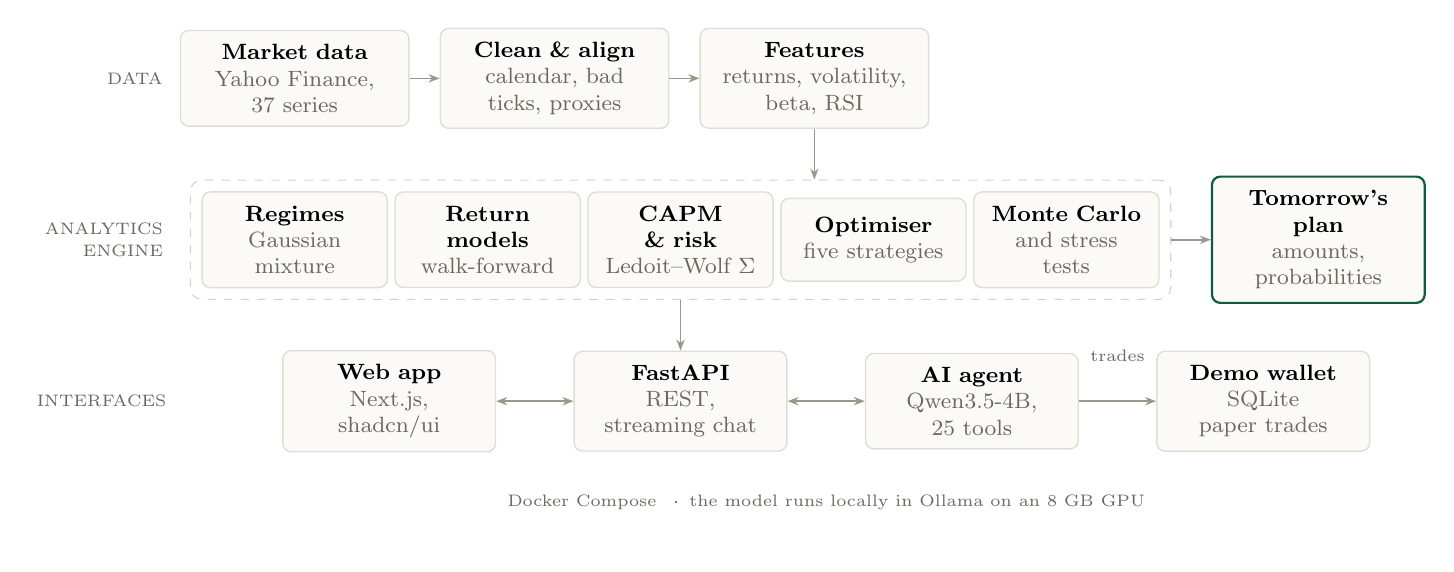
\begin{tikzpicture}[x=1cm, y=1cm, every node/.append style={minimum height=1.05cm}]
    % layer labels
    \node[lab, anchor=east, text width=1.6cm, align=right] at (-1.55, 0) {DATA};
    \node[lab, anchor=east, text width=1.6cm, align=right] at (-1.55, -2.05) {ANALYTICS\\ ENGINE};
    \node[lab, anchor=east, text width=1.6cm, align=right] at (-1.55, -4.1) {INTERFACES};
    % row 1: data
    \node[box, text width=2.55cm] (data)  at (0, 0)    {\textbf{Market data}\\\muted{Yahoo Finance, 37 series}};
    \node[box, text width=2.55cm] (clean) at (3.3, 0)  {\textbf{Clean \& align}\\\muted{calendar, bad ticks, proxies}};
    \node[box, text width=2.55cm] (feat)  at (6.6, 0)  {\textbf{Features}\\\muted{returns, volatility, beta, RSI}};
    % row 2: engine
    \node[box, text width=2.0cm] (reg)  at (0, -2.05)    {\textbf{Regimes}\\\muted{Gaussian mixture}};
    \node[box, text width=2.0cm] (ml)   at (2.45, -2.05) {\textbf{Return models}\\\muted{walk-forward}};
    \node[box, text width=2.0cm] (capm) at (4.9, -2.05)  {\textbf{CAPM \& risk}\\\muted{Ledoit--Wolf $\Sigma$}};
    \node[box, text width=2.0cm] (opt)  at (7.35, -2.05) {\textbf{Optimiser}\\\muted{five strategies}};
    \node[box, text width=2.0cm] (mc)   at (9.8, -2.05)  {\textbf{Monte Carlo}\\\muted{and stress tests}};
    \node[fit=(reg)(mc), draw=rulec, dashed, rounded corners=4pt, inner sep=4pt, minimum height=0pt] (eng) {};
    \node[hl, text width=2.35cm] (plan) at (13.0, -2.05) {\textbf{Tomorrow's plan}\\\muted{amounts, probabilities}};
    % row 3: interfaces
    \node[box, text width=2.35cm] (web)    at (1.2, -4.1)  {\textbf{Web app}\\\muted{Next.js, shadcn/ui}};
    \node[box, text width=2.35cm] (api)    at (4.9, -4.1)  {\textbf{FastAPI}\\\muted{REST, streaming chat}};
    \node[box, text width=2.35cm] (agent)  at (8.6, -4.1)  {\textbf{AI agent}\\\muted{Qwen3.5-4B, 25 tools}};
    \node[box, text width=2.35cm] (wallet) at (12.3, -4.1) {\textbf{Demo wallet}\\\muted{SQLite paper trades}};
    % flows
    \draw[flow] (data) -- (clean);
    \draw[flow] (clean) -- (feat);
    \draw[flow] (feat.south) -- (feat.south |- eng.north);
    \draw[flow] (eng.east) -- (plan.west);
    \draw[flow] (eng.south -| api.north) -- (api.north);
    \draw[flow, {Stealth[length=4pt]}-{Stealth[length=4pt]}] (web) -- (api);
    \draw[flow, {Stealth[length=4pt]}-{Stealth[length=4pt]}] (api) -- (agent);
    \draw[flow] (agent) -- node[lab, above=1pt]{trades} (wallet);
    \node[lab, anchor=north] at (6.75, -4.85) {Docker Compose \enspace·\enspace the model runs locally in Ollama on an 8 GB GPU};
  \end{tikzpicture}
\end{frame}

\begin{frame}{Data: Indian markets, 2014–2026}
  \vspace{0.15cm}
  \begin{columns}[T]
    \column{0.52\textwidth}
      \small
      \begin{tabularx}{\linewidth}{@{}Lr@{}}
        \toprl
        \thd{Universe} & \thd{Count}\\ \tabrule
        NSE stocks across 12 sectors (NIFTY 50 members) & 26\\
        Index ETFs: NIFTY 50, Next 50, Bank & 3\\
        Gold ETF \;·\; G-Sec bond ETF \;·\; liquid fund & 3\\ \tabrule
        Benchmark: NIFTY 50 index & 1\\
        Macro: India VIX, Brent, USD/INR, US 10Y, Bank NIFTY & 5\\ \botrl
      \end{tabularx}
      \vspace{0.35cm}

      \begin{columns}[T]
        \column{0.33\linewidth}\kpi{2,950}{trading days}
        \column{0.33\linewidth}\kpi{32}{investable assets}
        \column{0.33\linewidth}\kpi{12 yrs}{of daily OHLCV}
      \end{columns}
    \column{0.42\textwidth}
      \eyebrow{Data problems found and fixed}\par\vspace{3pt}\hair\par\vspace{5pt}
      \small
      \begin{itemize}\setlength{\itemsep}{5pt}
        \item \textbf{Wrong-scale prints} on 19--20 Dec 2019 in three ETFs (price $\div$10 to $\div$100) --- caught by a rolling-median filter.
        \item \textbf{Illiquid gilt ETF}: stale and erratic prints; tighter $\pm$4\% band around the 11-day median.
        \item \textbf{Liquid fund}: Yahoo's NAV ignores daily distributions; rebuilt from the RBI repo-rate path.
        \item All series aligned to the NSE trading calendar; small gaps forward-filled.
      \end{itemize}
  \end{columns}
\end{frame}

% ------------------------------------------------------------------ methods
\section{Methods}
\begin{frame}{Feature engineering}
  \vspace{0.2cm}
  \begin{columns}[T]
    \column{0.47\textwidth}
      \eyebrow{Per asset, strictly backward-looking}\par\vspace{3pt}\hair\par\vspace{5pt}
      \small
      \begin{itemize}\setlength{\itemsep}{3pt}
        \item Returns over 1, 5, 21, 63, 126, 252 days
        \item Realised volatility (21, 63 days) and their ratio
        \item Price vs 20/50-day averages; 50 vs 200-day
        \item RSI(14), MACD histogram, 252-day drawdown
        \item Rolling 63-day beta, correlation and skew vs NIFTY
      \end{itemize}
    \column{0.47\textwidth}
      \eyebrow{Market state (shared by all assets)}\par\vspace{3pt}\hair\par\vspace{5pt}
      \small
      \begin{itemize}\setlength{\itemsep}{3pt}
        \item NIFTY 21/63-day return, volatility, drawdown, gap to 200-day average
        \item India VIX level and 21-day change
        \item Brent, USD/INR and US 10-year moves
      \end{itemize}
      \vspace{0.25cm}
      \eyebrow{Target}\par\vspace{3pt}\hair\par\vspace{5pt}
      Forward 21-trading-day return of each asset \\[2pt]
      \muted{\footnotesize panel of 32 assets $\times$ 2,950 days}
  \end{columns}
\end{frame}

\begin{frame}{Market regimes}
  \framesubtitle{Gaussian mixture on NIFTY return, volatility, drawdown and India VIX}
  \vspace{0.05cm}
  \centering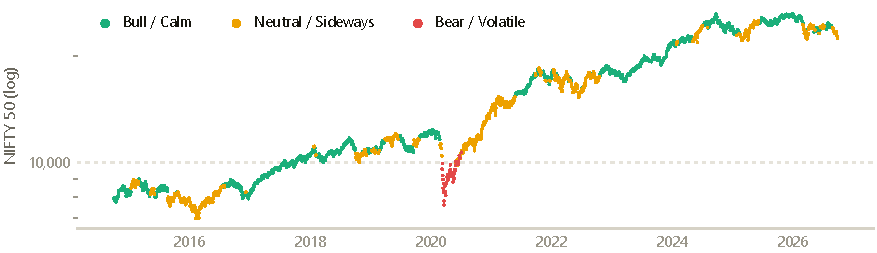
\includegraphics[width=\textwidth]{regimes.pdf}\par\vspace{0.1cm}\raggedright
  \footnotesize
  \begin{tabularx}{\textwidth}{@{}Lrrrrr@{}}
    \toprl
    \thd{Regime} & \thd{Share of days} & \thd{Return p.a.} & \thd{Volatility} & \thd{Avg VIX} & \thd{Persistence}\\ \tabrule
    \swatch{cC}\; Bull / Calm & 56\% & \up{+13.0\%} & 10.8\% & 13.6 & 96.3\%\\
    \swatch{cD}\; Neutral / Sideways \;\faint{(today)} & 42\% & \up{+6.5\%} & 17.6\% & 19.0 & 94.9\%\\
    \swatch{neg}\; Bear / Volatile & 2\% & +1.1\% & 54.5\% & 44.2 & 98.5\%\\ \botrl
  \end{tabularx}
\end{frame}

\begin{frame}{Forecasting returns, honestly}
  \framesubtitle{Expanding-window walk-forward, 2021--2026, purged targets; 43,400 out-of-sample predictions}
  \vspace{0.15cm}
  \begin{columns}[T]
    \column{0.56\textwidth}
      \small
      \begin{tabularx}{\linewidth}{@{}Lrrr@{}}
        \toprl
        \thd{Model} & \thd{RMSE} & \thd{Direction} & \thd{IC}\\ \tabrule
        Ridge regression \;\textcolor{brand}{\footnotesize in use} & 0.0566 & 51.2\% & 0.027\\
        Random Forest & 0.0572 & 50.6\% & 0.001\\
        XGBoost & 0.0583 & 50.4\% & $-$0.002\\ \tabrule
        \muted{Historical mean (baseline)} & \muted{0.0565} & \muted{47.5\%} & \muted{---}\\ \botrl
      \end{tabularx}\par\vspace{0.15cm}
      {\footnotesize\muted{IC = average daily Spearman correlation between forecast and realised return across assets.}}
    \column{0.38\textwidth}
      \begin{callout}
        \textbf{No model beats the naive baseline on error.} Cross-sectional skill is at most small (IC 0.00--0.03).\par\vspace{5pt}
        So the forecast is used only as a \emph{relative tilt}, weighted by measured skill:
        \[\lambda = \mathrm{clip}(5\cdot\mathrm{IC},\,0,\,0.5) = 13.5\%\]
        A model with no skill would get zero weight automatically.
      \end{callout}
  \end{columns}
\end{frame}

\begin{frame}{Volatility is forecastable; simulated outcomes are checked against reality}
  \vspace{0.15cm}
  \begin{columns}[T]
    \column{0.5\textwidth}
      \eyebrow{Next-month volatility, walk-forward 2021--26}\par\vspace{3pt}\hair\par\vspace{2pt}
      \small
      \begin{tabularx}{\linewidth}{@{}Lrr@{}}
        \toprl
        \thd{Model} & \thd{R$^2$} & \thd{Error}\\ \tabrule
        Ridge on range-based features \;\textcolor{brand}{\footnotesize in use} & 0.58 & 25\%\\
        \muted{Same as last quarter} & \muted{0.50} & \muted{29\%}\\
        \muted{Same as last month} & \muted{0.39} & \muted{31\%}\\ \botrl
      \end{tabularx}\par\vspace{0.2cm}
      {\footnotesize\muted{40{,}423 forecasts, settings chosen on 2019--20 only. Trees and ensembles scored lower. Liquid fund excluded.}}
    \column{0.46\textwidth}
      \eyebrow{Monte Carlo calibration, 1-year horizon}\par\vspace{3pt}\hair\par\vspace{2pt}
      \small
      \begin{itemize}\setlength{\itemsep}{4pt}
        \item 104 forecasts from quarterly dates 2019--25, information as of each date
        \item 90\% band held the outcome 81\% of the time (100\% in 2021--23, 44\% in 2020)
        \item The miss is the COVID crash and the rebound; realised returns beat expected by 7\% on average
        \item Reported as measured, not re-tuned to fit
      \end{itemize}
  \end{columns}
\end{frame}

\begin{frame}{Does the model stack create value? Walk-forward backtest, 2021--26}
  \vspace{0.1cm}
  \begin{columns}[T]
    \column{0.56\textwidth}
      \footnotesize
      \begin{tabularx}{\linewidth}{@{}Lrrrrr@{}}
        \toprl
        \thd{Strategy} & \thd{CAGR} & \thd{Vol} & \thd{Sharpe} & \thd{Max DD} & \thd{Turn./yr}\\ \tabrule
        Min-variance & 11.5\% & 5.7\% & 0.96 & $-$6.1\% & 0.8$\times$\\
        Max-Sharpe, prior & 12.8\% & 11.4\% & 0.60 & $-$16.1\% & 3.3$\times$\\
        \quad + volatility model & 14.5\% & 11.3\% & 0.75 & $-$15.2\% & 4.6$\times$\\
        \quad + 13.5\% return tilt & 15.3\% & 12.1\% & 0.77 & $-$16.5\% & 4.7$\times$\\
        \quad + regime overlay (full) & 14.1\% & 10.1\% & 0.80 & $-$13.6\% & 5.0$\times$\\ \tabrule
        \muted{NIFTY 50 ETF} & \muted{10.4\%} & \muted{12.8\%} & \muted{0.34} & \muted{$-$16.1\%} & \muted{0.2$\times$}\\
        \muted{Equal-weight stocks} & \muted{16.6\%} & \muted{13.0\%} & \muted{0.82} & \muted{$-$15.0\%} & \muted{0.7$\times$}\\ \botrl
      \end{tabularx}\par\vspace{0.12cm}
      {\footnotesize\muted{Monthly rebalance, long-only, 0.10\% cost per trade; every input uses only data available at each date.}}
    \column{0.42\textwidth}
      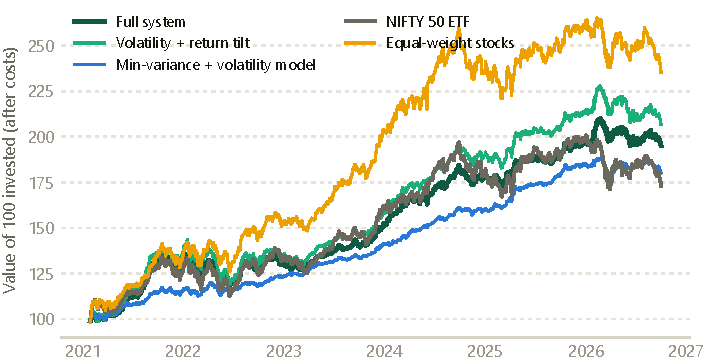
\includegraphics[width=\linewidth]{eval_curves.pdf}\par\vspace{0.08cm}
      \begin{callout}
        The volatility model and regime overlay add \emph{risk control}; the return tilt adds little. An equal-weight stock basket matches the full system in this one bull-market sample.
      \end{callout}
  \end{columns}
\end{frame}

\begin{frame}{Robustness: year by year, calibration, and what regimes and anomalies tell us}
  \vspace{0.1cm}
  \begin{columns}[T]
    \column{0.5\textwidth}
      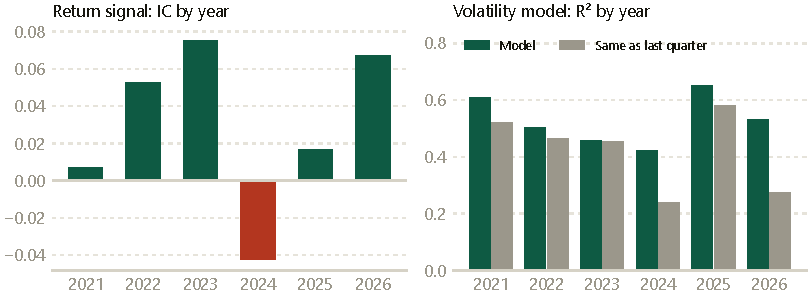
\includegraphics[width=\linewidth]{eval_by_year.pdf}\par\vspace{0.1cm}
      {\footnotesize\muted{Return signal: IC positive in 5 of 6 years, never significant on its own. Volatility model: ahead of the baseline in 5 of 6 years, tied in 2023.}}
    \column{0.46\textwidth}
      \small
      \begin{itemize}\setlength{\itemsep}{5pt}
        \item \textbf{Calibration.} Intervals of 50 / 75 / 90 / 95 / 99\% held 44 / 69 / 81 / 84 / 93\%. Fatter tails or a block bootstrap do not fix it: the miss is the 2020 crash.
        \item \textbf{Regimes.} Calm $\to$ Neutral in a month 18\% of the time. After Neutral, 35\% of months saw a $\ge$5\% market drawdown against 13\% after Calm. They do not improve the volatility forecast (VIX already carries it).
        \item \textbf{Anomalies.} Flagged days are followed by 21--23\% volatility vs 13\% and a 5\% drawdown 60--65\% of the time vs 21\%, but not by lower returns: a risk warning, not a sell signal.
        \item \textbf{Return signal.} Relative-strength features lift IC to 0.04 (not significant on independent windows): a candidate, not adopted.
      \end{itemize}
  \end{columns}
\end{frame}

\begin{frame}{Expected returns and the risk model}
  \vspace{0.15cm}
  \begin{columns}[T]
    \column{0.5\textwidth}
      \eyebrow{CAPM}\par\vspace{3pt}\hair\par\vspace{2pt}
      \[ \mathbb{E}[R_i] = r_f + \beta_i\,\mathrm{ERP}, \qquad r_f = 6\% \]
      {\small ERP blends 5-year NIFTY history with a 5.5\% prior, clipped to [3\%, 8\%] $\Rightarrow$ 3.0\%, market return 9.0\%.}\par\vspace{0.25cm}
      \eyebrow{Final expected return}\par\vspace{3pt}\hair\par\vspace{2pt}
      \[ \mu_i = 0.6\,\mathrm{CAPM}_i + 0.4\,\mathrm{History}_i + \lambda\cdot\mathrm{Tilt}^{\mathrm{ML}}_i \]
    \column{0.44\textwidth}
      \eyebrow{Risk}\par\vspace{3pt}\hair\par\vspace{4pt}
      \small
      \begin{itemize}\setlength{\itemsep}{4pt}
        \item Covariance $\Sigma$: Ledoit--Wolf shrinkage on 5 years of daily returns
        \item $\mathrm{VaR}_{95}$ and $\mathrm{CVaR}_{95} = \mathbb{E}[L \mid L \ge \mathrm{VaR}]$
        \item Maximum drawdown, Sharpe $=(\mu-r_f)/\sigma$
        \item Oil and rate sensitivities for stress tests
        \item Isolation Forest flags anomalous market days
      \end{itemize}
  \end{columns}
\end{frame}

\begin{frame}{Five strategies on one efficient frontier}
  \vspace{0.05cm}
  \begin{columns}[T]
    \column{0.47\textwidth}
      \footnotesize
      \begin{tabularx}{\linewidth}{@{}p{2.85cm}L@{}}
        \toprl
        \thd{Strategy} & \thd{Optimisation}\\ \tabrule
        \swatch{cB}\; Max Return & $\max_w\, w^\top\mu$ \;(linear program)\\
        \swatch{cA}\; Min Risk & $\min_w\, w^\top\Sigma w$\\
        \swatch{cC}\; Max Sharpe & $\max_w\, (w^\top\mu - r_f)/\sqrt{w^\top\Sigma w}$\\
        \swatch{cG}\; Goal-Based & frontier point with the highest \emph{simulated} P(reach target)\\
        \swatch{cE}\; Crash-Resistant & $\min\mathrm{CVaR}_{95}$ over history \emph{and} stress scenarios (Rockafellar--Uryasev LP)\\ \botrl
      \end{tabularx}\par\vspace{0.2cm}
      {\footnotesize\muted{Long-only, fully invested; per-asset caps by risk profile (single stock 8 / 15 / 25\%); preferred sectors restrict the stock universe.}}
    \column{0.5\textwidth}
      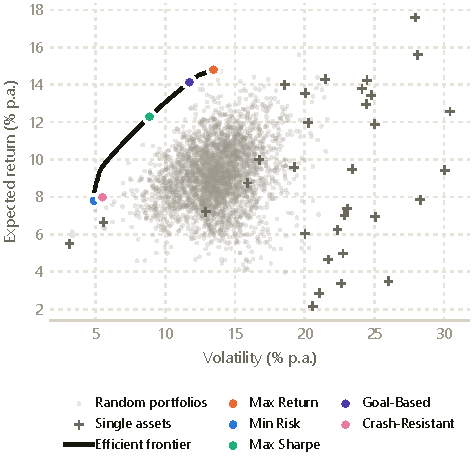
\includegraphics[width=0.86\linewidth]{frontier.pdf}
  \end{columns}
\end{frame}

\begin{frame}{Monte Carlo engine}
  \vspace{0.05cm}
  \begin{columns}[T]
    \column{0.42\textwidth}
      \small
      \begin{itemize}\setlength{\itemsep}{5pt}
        \item \textbf{10,000 daily paths} per strategy over the horizon
        \item \textbf{Fat tails}: Student-$t$ innovations, $\nu = 5$
        \item \textbf{Regime switching}: 3-state Markov chain from the GMM transition matrix, started from today's regime
        \item Drift $\ln(1+\mu) - \tfrac12\sigma_k^2$ so the mean equals the expected return
        \item \textbf{Day-0 shocks} move the market into the bear regime
        \item Outputs: P(gain), P(target), VaR, CVaR, drawdowns, percentile bands
      \end{itemize}
    \column{0.55\textwidth}
      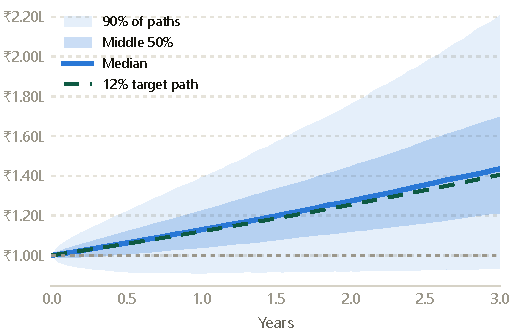
\includegraphics[width=\linewidth]{fan.pdf}\par
      {\footnotesize\muted{Recommended plan, ₹1,00,000 over 3 years: median, middle 50\% and 90\% of paths against the 12\% target path.}}
  \end{columns}
\end{frame}

% ------------------------------------------------------------------ results
\section{Results}
\begin{frame}{Tomorrow's investment plan}
  \framesubtitle{Sample investor: ₹1,00,000 \;·\; 3 years \;·\; medium risk \;·\; 12\% target \;·\; prices at the close of 1 Oct 2026}
  \vspace{0.1cm}
  \begin{columns}[T]
    \column{0.47\textwidth}
      {\displayfont\fontsize{19}{22}\selectfont Goal-Based \; {\fontsize{7}{8}\selectfont\sffamily\color{brand}\addfontfeature{LetterSpace=10}RECOMMENDED}\par}\vspace{3pt}
      {\footnotesize\muted{Within medium-risk limits and the best chance (58\%) of reaching 12\%; ties within 2 pp go to the higher Sharpe.}}\par\vspace{0.2cm}
      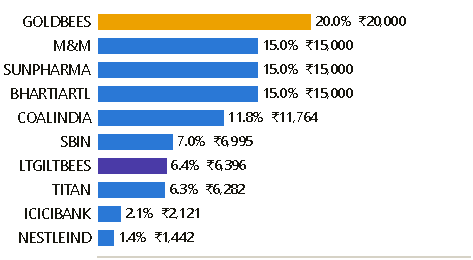
\includegraphics[width=0.96\linewidth]{allocation.pdf}\par
      {\footnotesize\swatch{cA}\,Stocks 76\% \quad \swatch{cD}\,Gold 20\% \quad \swatch{faint}\,Cash \faint{\& residual}}
    \column{0.47\textwidth}
      \vspace{0.35cm}
      \begin{columns}[T]
        \column{0.5\linewidth}\kpi{14.4\%}{Expected return}\par\vspace{9pt}\kpi{96\%}{Chance of gain}\par\vspace{9pt}\kpi{14.5\%}{Expected drawdown}
        \column{0.5\linewidth}\kpi{12.9\%}{Volatility}\par\vspace{9pt}\kpi{58\%}{Reach 12\% target}\par\vspace{9pt}\kpi{8 of 9}{Stress tests passed}
      \end{columns}
      \vspace{0.3cm}\hair\par\vspace{3pt}
      {\footnotesize Sharpe 0.65 \;·\; beta 0.74 \;·\; 1-year VaR\textsubscript{95} 7.3\% \;·\; CVaR\textsubscript{95} 13.9\%\par
       \muted{Whole shares at the latest close, after 0.1\% trading costs.}}
  \end{columns}
\end{frame}

\begin{frame}{What could happen: the distribution, not a point}
  \vspace{0.05cm}
  \begin{columns}[T]
    \column{0.55\textwidth}
      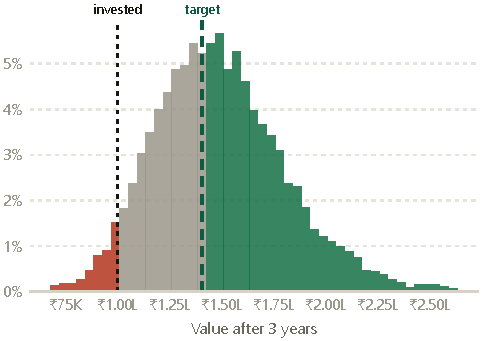
\includegraphics[width=\linewidth]{distribution.pdf}\par
      {\footnotesize\swatch{pos}\;target met \quad\swatch{faint}\;gain, below target \quad\swatch{neg}\;loss}
    \column{0.4\textwidth}
      \vspace{0.2cm}
      \eyebrow{Value after 3 years}\par\vspace{3pt}\hair\par\vspace{4pt}
      \begin{tabularx}{\linewidth}{@{}Lr@{}}
        Worst 5\% & {\numfont ₹1,01,941}\\
        \textbf{Median} & {\numfont\textbf{₹1,46,925}}\\
        Best 5\% & {\numfont ₹2,06,622}\\
      \end{tabularx}\par\vspace{0.3cm}
      \eyebrow{Proposal's illustration vs system output}\par\vspace{3pt}\hair\par\vspace{2pt}
      \footnotesize
      \begin{tabularx}{\linewidth}{@{}Lrr@{}}
        & \thd{Proposal} & \thd{System}\\
        Expected return & $\sim$12.4\% & 14.4\%\\
        Volatility & $\sim$14.2\% & 12.9\%\\
        P(positive) & $\sim$73\% & 96\%\\
        P(target) & $\sim$68\% & 58\%\\
      \end{tabularx}
  \end{columns}
\end{frame}

\begin{frame}{Five strategies compared}
  \framesubtitle{Same investor, same 10,000 simulated futures for every strategy}
  \vspace{0.25cm}
  \small
  \begin{tabularx}{\textwidth}{@{}Lrrrrrr@{}}
    \toprl
    \thd{Strategy} & \thd{Return} & \thd{Volatility} & \thd{Sharpe} & \thd{Chance of gain} & \thd{Reach target} & \thd{Median value}\\ \tabrule
    \swatch{cB}\; Max Return & 14.8\% & 14.2\% & 0.62 & 94\% & \textbf{58\%} & ₹1,47,461\\
    \swatch{cA}\; Min Risk & 7.1\% & 4.9\% & 0.22 & 99\% & 4\% & ₹1,22,476\\
    \swatch{cC}\; Max Sharpe & 12.4\% & 9.5\% & \textbf{0.67} & 98\% & 50\% & ₹1,40,605\\
    \swatch{cG}\; \textbf{Goal-Based} \;\textcolor{brand}{\footnotesize recommended} & 14.4\% & 12.9\% & 0.65 & 96\% & \textbf{58\%} & ₹1,46,925\\
    \swatch{cE}\; Crash-Resistant & 7.4\% & 5.5\% & 0.25 & 99\% & 7\% & ₹1,23,409\\ \botrl
  \end{tabularx}
  \vspace{0.45cm}
  \begin{callout}
    \textbf{Decision rule.} Keep strategies inside the investor's limits on volatility, worst stress loss and one-year VaR;
    pick the highest probability of reaching the target; within 2 percentage points prefer the higher Sharpe ratio.
    Defensive strategies are almost certain to gain but rarely reach a 12\% goal.
  \end{callout}
\end{frame}

\begin{frame}{Stress tests}
  \vspace{0.05cm}
  \begin{columns}[T]
    \column{0.58\textwidth}
      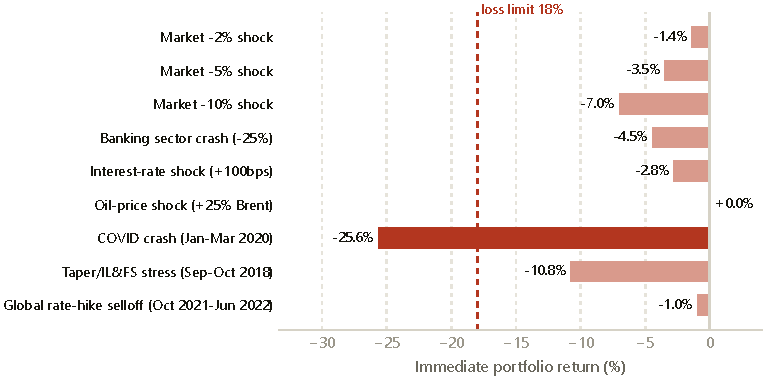
\includegraphics[width=\linewidth]{stress.pdf}
    \column{0.37\textwidth}
      \eyebrow{Monte Carlo after a day-0 shock}\par\vspace{3pt}\hair\par\vspace{3pt}
      \footnotesize
      \begin{tabularx}{\linewidth}{@{}Lrr@{}}
        \thd{Scenario} & \thd{Median} & \thd{P(tgt)}\\
        No shock & ₹1,47,278 & 59\%\\
        Market $-$2\% & ₹1,45,088 & 56\%\\
        Market $-$5\% & ₹1,37,454 & 47\%\\
        Market $-$10\% & ₹1,32,146 & 41\%\\
        Pharma crash & ₹1,36,467 & 46\%\\
        Rate +100 bp & ₹1,38,899 & 48\%\\
        Oil +25\% & ₹1,47,545 & 60\%\\
      \end{tabularx}\par\vspace{0.2cm}
      {\footnotesize\muted{Only a COVID-scale crash (\dn{$-$26.8\%}) breaches the 18\% medium-risk loss limit.}}
  \end{columns}
\end{frame}

\begin{frame}{Invest now, wait, or SIP?}
  \framesubtitle{All options run on the same simulated markets; uninvested money earns the risk-free rate}
  \vspace{0.25cm}
  \begin{columns}[T]
    \column{0.56\textwidth}
      \small
      \begin{tabularx}{\linewidth}{@{}Lrr@{}}
        \toprl
        \thd{Option} & \thd{Median after 3 yr} & \thd{Beats lump sum}\\ \tabrule
        \textbf{Invest now (lump sum)} & \textbf{₹1,46,205} & ---\\
        Wait 1 month & ₹1,45,444 & 44\%\\
        Wait 3 months & ₹1,43,725 & 38\%\\
        Wait 6 months & ₹1,41,197 & 34\%\\
        SIP over 6 months & ₹1,44,301 & 37\%\\
        SIP over 12 months & ₹1,42,120 & 32\%\\ \botrl
      \end{tabularx}
    \column{0.38\textwidth}
      \vspace{0.2cm}
      \begin{callout}
        With a positive expected return, \textbf{time in the market beats timing it}: every delay lowers the median outcome.\par\vspace{5pt}
        A SIP is still useful when the investor values a narrower range of bad outcomes over the higher median --- it wins in about a third of futures.
      \end{callout}
  \end{columns}
\end{frame}

\begin{frame}{Walk-forward backtest}
  \framesubtitle{Weights chosen only from data before 3 Oct 2023, rebalanced quarterly, held to 1 Oct 2026; no ML (no look-ahead)}
  \vspace{0.05cm}
  \centering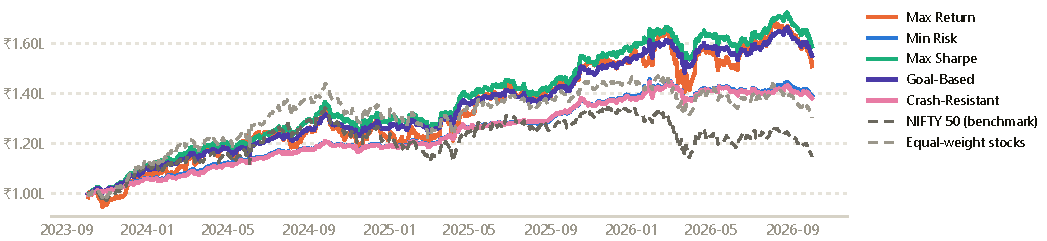
\includegraphics[width=\textwidth]{backtest.pdf}\par\vspace{0.05cm}\raggedright
  \footnotesize
  \begin{tabularx}{\textwidth}{@{}Lrrrrr@{}}
    \toprl
    \thd{Strategy} & \thd{Total return} & \thd{CAGR} & \thd{Volatility} & \thd{Sharpe} & \thd{Max drawdown}\\ \tabrule
    \swatch{cG}\; Goal-Based & \up{+55.1\%} & 16.1\% & 8.9\% & \textbf{1.14} & $-$8.1\%\\
    \swatch{cC}\; Max Sharpe & \up{+58.8\%} & 17.1\% & 10.3\% & 1.07 & $-$9.3\%\\
    \swatch{cA}\; Min Risk \;/\; \swatch{cE}\; Crash-Resistant & \up{+39.1\%} \;/\; \up{+38.1\%} & 11.9 / 11.6\% & 5.9 / 6.0\% & 1.00 / 0.95 & $-$6.8 / $-$6.3\%\\
    \muted{NIFTY 50 benchmark} & \muted{+14.8\%} & \muted{4.8\%} & \muted{13.3\%} & \muted{$-$0.09} & \muted{$-$15.8\%}\\ \botrl
  \end{tabularx}
\end{frame}

% ------------------------------------------------------------------ agent
\section{AI agent}
\begin{frame}{The agent: Qwen3.5-4B with tools}
  \framesubtitle{Runs locally through Ollama; the language model chooses tools and explains, the engine produces every number}
  \vspace{0.0cm}
  \centering
  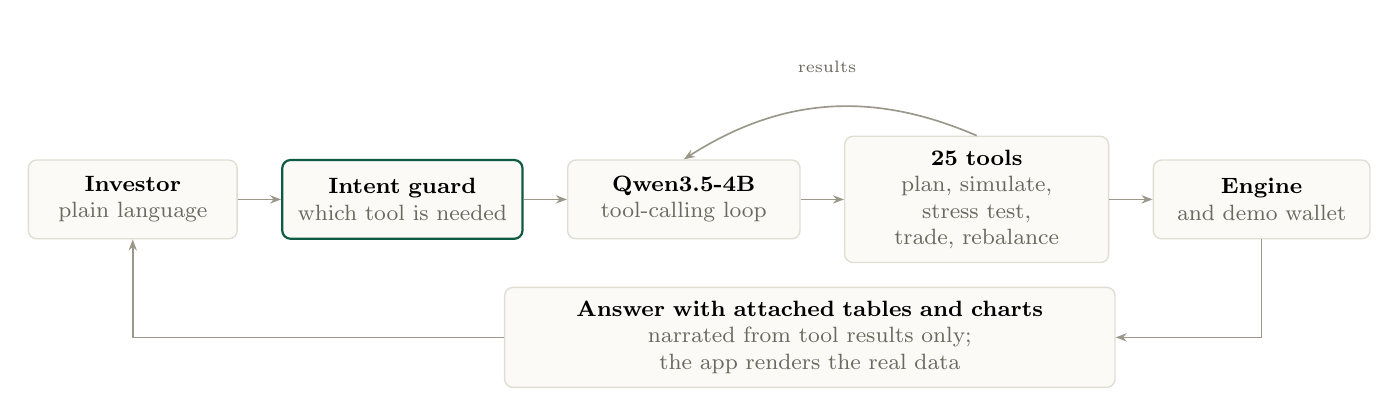
\begin{tikzpicture}[node distance=0.5cm]
    \tikzset{every node/.append style={minimum height=1.0cm}}
    \node[box, text width=2.3cm] (u) {\textbf{Investor}\\\muted{plain language}};
    \node[hl, text width=2.7cm, right=0.55cm of u] (g) {\textbf{Intent guard}\\\muted{which tool is needed}};
    \node[box, text width=2.6cm, right=0.55cm of g] (l) {\textbf{Qwen3.5-4B}\\\muted{tool-calling loop}};
    \node[box, text width=3.0cm, right=0.55cm of l] (t) {\textbf{25 tools}\\\muted{plan, simulate, stress test,\\ trade, rebalance}};
    \node[box, text width=2.4cm, right=0.55cm of t] (e) {\textbf{Engine}\\\muted{and demo wallet}};
    \node[box, text width=7.4cm, below=0.6cm of l, xshift=1.6cm] (o) {\textbf{Answer with attached tables and charts}\\\muted{narrated from tool results only; the app renders the real data}};
    \draw[flow] (u)--(g); \draw[flow] (g)--(l); \draw[flow] (l)--(t); \draw[flow] (t)--(e);
    \draw[flow] (e.south) |- (o.east);
    \draw[flow] (t.north) to[bend right=28] node[lab, above]{results} (l.north);
    \draw[flow] (o.west) -| (u.south);
  \end{tikzpicture}
  \vspace{0.1cm}
  \begin{columns}[T]
    \column{0.31\textwidth}
      \eyebrow{Grounding}\par\vspace{3pt}\hair\par\vspace{3pt}
      {\footnotesize Early tests: the 4B model invented an allocation. Now, if a request needs a tool and the model skips it, the agent runs it and the model only narrates.}
    \column{0.31\textwidth}
      \eyebrow{Guards in code}\par\vspace{3pt}\hair\par\vspace{3pt}
      {\footnotesize A strategy sticks only if the user named it; trades need an instruction, not a question; resets need an explicit “reset”.}
    \column{0.31\textwidth}
      \eyebrow{Measured}\par\vspace{3pt}\hair\par\vspace{3pt}
      {\footnotesize \textbf{23 / 23} scripted conversation cases pass, covering analysis, trading, stop-loss handling and ask-first confirmation.}
  \end{columns}
\end{frame}

\begin{frame}{Autonomous trading with demo money}
  \vspace{0.15cm}
  \begin{columns}[T]
    \column{0.47\textwidth}
      \eyebrow{Two modes}\par\vspace{3pt}\hair\par\vspace{4pt}
      \small
      \textbf{Auto-trade} --- “invest it”, “sell all my TCS”, “rebalance” execute immediately. \emph{Questions never trade}: “should I sell TCS?” gets analysis.\par\vspace{5pt}
      \textbf{Ask first} --- every order is staged; it executes only after the investor's own “confirm”.\par\vspace{0.3cm}
      \eyebrow{Demo wallet}\par\vspace{3pt}\hair\par\vspace{4pt}
      ₹10,00,000 of virtual cash in SQLite; fills at the latest close with 0.05\% brokerage + 0.05\% slippage; atomic multi-order execution.
    \column{0.47\textwidth}
      \eyebrow{Health check \& auto-manage}\par\vspace{3pt}\hair\par\vspace{2pt}
      \footnotesize
      \begin{tabularx}{\linewidth}{@{}p{2.1cm}L@{}}
        \textbf{Stop-loss} & position down 15\% from cost $\Rightarrow$ sell\\ \tabrule
        \textbf{Drift} & holding above its cap by 3 pp $\Rightarrow$ trim\\ \tabrule
        \textbf{Risk limit} & volatility $>$ 1.1$\times$ limit $\Rightarrow$ de-risk\\ \tabrule
        \textbf{Bear regime} & equity $>$ 60\% $\Rightarrow$ move to Crash-Resistant\\ \tabrule
        \textbf{Idle cash} & $>$ 25\% of wallet $\Rightarrow$ deploy\\
      \end{tabularx}\par\vspace{0.2cm}
      {\footnotesize\muted{\textbf{Autopilot} runs this review when switched on and after every market-data refresh.}}
  \end{columns}
\end{frame}

% ------------------------------------------------------------------ app
\section{Application}
\begin{frame}{Web application: the planner}
  \framesubtitle{Next.js 16, TypeScript, Tailwind CSS, shadcn/ui \;·\; screenshot of the running app (data refreshed 2 Oct 2026)}
  \vspace{0.1cm}
  \centering\shot{height=6.55cm, trim=0 400 0 0, clip}{ui/planner.png}\par\vspace{0.12cm}
  \raggedright{\footnotesize\muted{Profile on the left; the five strategies; the recommended plan with its key figures, risk-limit check, allocation and composition. Tabs open the Monte Carlo, stress tests, timing and backtest views.}}
\end{frame}

\begin{frame}{Web application: overview, agent, markets, portfolio}
  \vspace{0.05cm}
  \begin{columns}[T,totalwidth=\textwidth]
    \column{0.49\textwidth}
      \eyebrow{Overview}\par\vspace{2pt}\shot{width=\linewidth, trim=0 560 0 0, clip}{ui/overview.png}\par\vspace{0.22cm}
      \eyebrow{Markets}\par\vspace{2pt}\shot{width=\linewidth, trim=0 560 0 0, clip}{ui/market.png}
    \column{0.49\textwidth}
      \eyebrow{Agent}\par\vspace{2pt}\shot{width=\linewidth, trim=0 560 0 0, clip}{ui/agent.png}\par\vspace{0.22cm}
      \eyebrow{Portfolio}\par\vspace{2pt}\shot{width=\linewidth, trim=0 560 0 0, clip}{ui/wallet.png}
  \end{columns}
\end{frame}

\begin{frame}{Engineering and verification}
  \vspace{0.15cm}
  \begin{columns}[T]
    \column{0.31\textwidth}
      \eyebrow{Stack}\par\vspace{3pt}\hair\par\vspace{4pt}
      \footnotesize
      Python 3.13 \;·\; pandas, scikit-learn, XGBoost, PyTorch, SciPy\par\vspace{3pt}
      FastAPI with streaming chat\par\vspace{3pt}
      Ollama + Qwen3.5-4B (RTX 4070, 8 GB)\par\vspace{3pt}
      Next.js 16, TypeScript, Tailwind, shadcn/ui, Recharts\par\vspace{3pt}
      Docker Compose (API + web)
    \column{0.31\textwidth}
      \kpi{55}{unit tests passing}\par\vspace{9pt}
      \kpi{27}{API endpoint checks}\par\vspace{9pt}
      \kpi{23 / 23}{agent conversation cases}
    \column{0.31\textwidth}
      \eyebrow{What the tests cover}\par\vspace{3pt}\hair\par\vspace{4pt}
      \footnotesize
      CAPM, VaR/CVaR and drawdown maths; optimiser constraints for every risk level; Monte Carlo mean and shock behaviour; wallet accounting;
      trade intent detection; confirmation and stop-loss guards.\par\vspace{0.35cm}
      \muted{Code: github.com/Tendool/If-I-invest-tomorrow}
  \end{columns}
\end{frame}

% ------------------------------------------------------------------ close
\section{Close}
\begin{frame}{Limitations}
  \vspace{0.2cm}
  \begin{columns}[T]
    \column{0.47\textwidth}
      \small
      \begin{itemize}\setlength{\itemsep}{6pt}
        \item \textbf{Weak predictability}: monthly returns are close to unforecastable; the ML adds only a small tilt.
        \item \textbf{Assumptions}: risk-free rate 6\%, ERP prior, sector rate sensitivities and bond duration are set by hand.
        \item \textbf{One backtest window}: NIFTY was weak over 2023--26 in this data, which flatters diversified portfolios.
      \end{itemize}
    \column{0.47\textwidth}
      \small
      \begin{itemize}\setlength{\itemsep}{6pt}
        \item \textbf{Data}: Yahoo Finance prices; the liquid fund is a reconstructed proxy; no taxes (STT, capital gains).
        \item \textbf{Small language model}: occasional slips in wording; the tables under each answer are authoritative.
        \item \textbf{Simulation only}: demo money, not investment advice.
      \end{itemize}
  \end{columns}
\end{frame}

\begin{frame}{Future work}
  \vspace{0.2cm}
  \begin{columns}[T]
    \column{0.31\textwidth}
      \eyebrow{Signals}\par\vspace{3pt}\hair\par\vspace{4pt}
      \small News sentiment with FinBERT as a model feature; macro factors from RBI data; Black--Litterman views instead of a fixed blend.
    \column{0.31\textwidth}
      \eyebrow{Realism}\par\vspace{3pt}\hair\par\vspace{4pt}
      \small Indian tax and transaction costs; mutual funds and SIP products; multi-period rebalancing; intraday data.
    \column{0.31\textwidth}
      \eyebrow{Agent}\par\vspace{3pt}\hair\par\vspace{4pt}
      \small Benchmark 7--9B local models on the same 23 cases; scheduled autopilot; explanation of each trade in the history.
  \end{columns}
\end{frame}

\begin{frame}{Conclusion}
  \vspace{0.3cm}
  {\displayfont\fontsize{19}{25}\selectfont From \emph{“what might happen”} to \emph{“what to do tomorrow”}.\par}
  \vspace{0.45cm}
  \begin{columns}[T]
    \column{0.31\textwidth}
      \kpi[brand]{1}{integrated pipeline}\par\vspace{4pt}
      {\footnotesize Data, ML, CAPM, optimisation, Monte Carlo and stress testing in one system.}
    \column{0.31\textwidth}
      \kpi[brand]{5}{strategies, one rule}\par\vspace{4pt}
      {\footnotesize Compared on the same futures and chosen transparently against the investor's limits.}
    \column{0.31\textwidth}
      \kpi[brand]{1}{agent that acts}\par\vspace{4pt}
      {\footnotesize Plans, simulates, invests, sells and rebalances --- grounded in the engine, guarded in code.}
  \end{columns}
  \vspace{0.5cm}
  \begin{callout}
    The honest finding matters as much as the plan: forecasting single-month returns barely beats a naive baseline, so the
    value of the system lies in measuring risk, comparing strategies and showing the full range of outcomes.
  \end{callout}
\end{frame}

\begin{frame}{References}
  \vspace{0.1cm}
  \footnotesize
  \begin{enumerate}\setlength{\itemsep}{2.5pt}
    \item Markowitz, H. --- Portfolio Selection. \emph{Journal of Finance}, 1952.
    \item Sharpe, W. F. --- Capital Asset Prices: A Theory of Market Equilibrium under Conditions of Risk. \emph{Journal of Finance}, 1964.
    \item Glasserman, P. --- \emph{Monte Carlo Methods in Financial Engineering}. Springer, 2004.
    \item Hull, J. C. --- \emph{Options, Futures, and Other Derivatives}. Pearson.
    \item Hochreiter, S. \& Schmidhuber, J. --- Long Short-Term Memory. \emph{Neural Computation}, 1997.
    \item Ledoit, O. \& Wolf, M. --- A Well-Conditioned Estimator for Large-Dimensional Covariance Matrices. \emph{Journal of Multivariate Analysis}, 2004.
    \item Rockafellar, R. T. \& Uryasev, S. --- Optimization of Conditional Value-at-Risk. \emph{Journal of Risk}, 2000.
    \item Hamilton, J. D. --- A New Approach to the Economic Analysis of Nonstationary Time Series and the Business Cycle. \emph{Econometrica}, 1989.
    \item Liu, F. T., Ting, K. M. \& Zhou, Z.-H. --- Isolation Forest. \emph{IEEE ICDM}, 2008.
    \item Chen, T. \& Guestrin, C. --- XGBoost: A Scalable Tree Boosting System. \emph{KDD}, 2016.
    \item Cho, K. et al. --- Learning Phrase Representations using RNN Encoder--Decoder (GRU). \emph{EMNLP}, 2014.
  \end{enumerate}
\end{frame}

\begin{frame}[plain]
  \vspace*{2.2cm}
  \hspace*{0.15cm}\begin{minipage}{0.9\textwidth}
    {\displayfont\fontsize{38}{40}\selectfont Thank \textit{you}\par}\vspace{0.3cm}
    {\fontsize{13}{16}\selectfont\color{muted}Questions and live demo\par}\vspace{0.7cm}
    {\color{rulec}\rule{\linewidth}{0.4pt}}\par\vspace{0.25cm}
    {\small\color{muted}Rupali K \enspace·\enspace Mahadev S \enspace·\enspace Srivatsav S \enspace·\enspace Sarang U \hfill github.com/Tendool/If-I-invest-tomorrow}
  \end{minipage}
\end{frame}

\end{document}
